  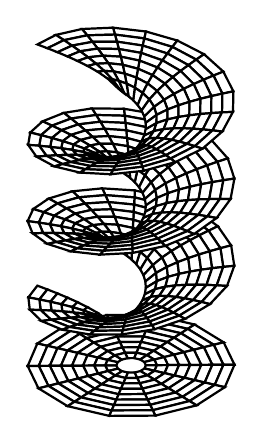
\begin{tikzpicture}[scale=2]
    \begin{axis}[
        axis lines=none,
        axis equal image,
        trig format plots=rad,
        z buffer=sort]
   \addplot3 [
        surf,
        domain=1:7,
        domain y=-pi:pi,
        samples=9,
        samples y=15,
        shader=flat,
        draw=black,
        fill=white
        ]
    ({x*cos(y)},{x*sin(y)},{-12});
   \addplot3 [
        surf,
        domain=1:7,
        samples=9,
        samples y=60,
        shader=flat,
        draw=black,
        fill=white,
        domain y=-3*pi:3*pi
        ]
    ({x*cos(y)},{x*sin(y)},{ln(x)+ y});
    \end{axis}
  \end{tikzpicture}


